The units and uncertainties of the properties in this section are set here. The energy unit is eV with uncertainty $\pm$ 0.003 eV, pressure is in units kbar with uncertainty $\pm$ 1 kbar and force in units eV/Å with uncertainty $\pm$ 0.01 eV/Å.

\subsection{Convergence}

We started by checking the convergence. The figures have some normal convergence criteria plotted with the results. 

\subsubsection{Energy cut-off}

\begin{equation}\label{eq:relative_energy}
|\Delta E_{rel}^i| =\left| \left( E_a^{i+1}-E_a^i\right)-\left( E_b^{i+1}-E_b^i\right)\right|
\end{equation}

We started with the energy convergence. Figure \ref{fig:totencutoff} shows the plot of the change in relative energy (Equation \ref{eq:relative_energy}) between the total energy of the unit cell, $E_a$, and the total energy of the unit cell with one less oxygen, $E_b$, against the cut-off energy. The plot shows that a cut-off energy of 600 eV would give a good convergence well below 1 meV for the energy.

\begin{figure}[H]
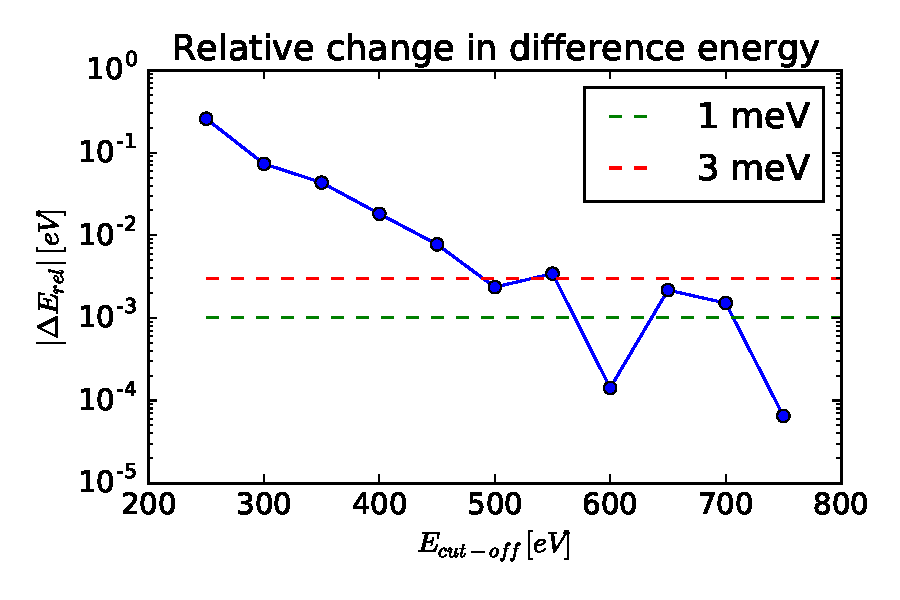
\includegraphics[width=\linewidth]{../fig/deltatotencurverel.pdf}\caption{This is a plot of the difference between change in energy for $\text{Ga}_2\text{O}_3$ with and without a oxygen vacancy. We can see from the plot that a cut-off energy of 600 eV is sufficient.}\label{fig:totencutoff}
\end{figure}

We also looked at the force and the pressure with respect to the cut-off energy. Figure \ref{fig:forcepresscutoff} shows the result. A cut-off energy of 600 eV gives a good convergence for force and pressure also. 

\begin{figure}[H]
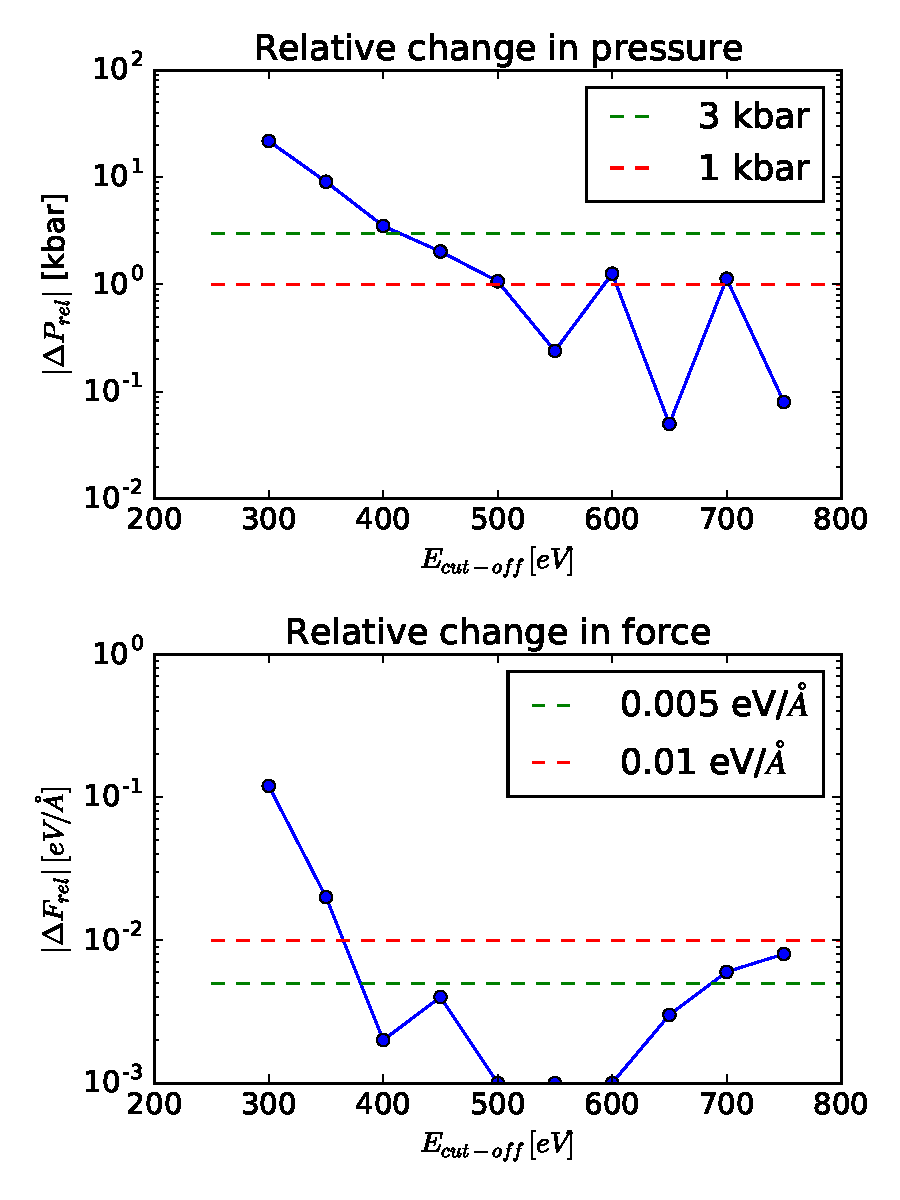
\includegraphics[width=\linewidth]{../fig/deltaforcepressrel.pdf}\caption{This is a plot of the difference between change in both force and pressure for $\text{Ga}_2\text{O}_3$ with and without a oxygen vacancy. We can see from the plot that with respect to pressure and force 600 eV is more than sufficient. The change in force increases, but it is still small.}\label{fig:forcepresscutoff}
\end{figure}

After increasing the primitive unit cell to a super cell, the CPU time of the relaxation increased a lot. To make the calculations more workable, the convergence criteria was made a little less strict and the new cut-off energy was sat to 500 eV. When we look at Figure \ref{fig:totencutoff} and \ref{fig:forcepresscutoff} we see that a cut-off energy at 500 eV gives a good convergence as well, it is still around 1-10 meV for the energy and around 1 kbar for the pressure and 0.005 eV/Å for the force.

\subsubsection{k-point density}

Thereafter, we evaluated the necessary k-point density. Figure \ref{fig:totenkpoints} shows the result for the relative change in energy and Figure \ref{fig:forcepresskpoints} force and pressure. 

\begin{figure}[H]
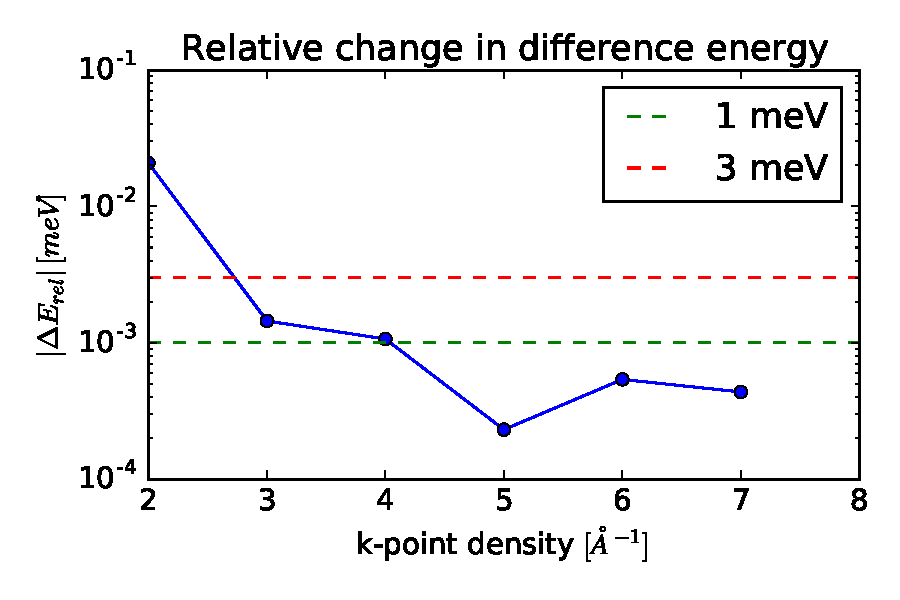
\includegraphics[width=\linewidth]{../fig/deltatotencurverel_kpoints.pdf}\caption{This is a plot of the difference between change in energy for $\text{Ga}_2\text{O}_3$ with and without a oxygen vacancy. We can see from the plot that a k-point density of 5 $\text{Å}^{-1}$ is sufficient.}\label{fig:totenkpoints}
\end{figure}

\begin{figure}[H]
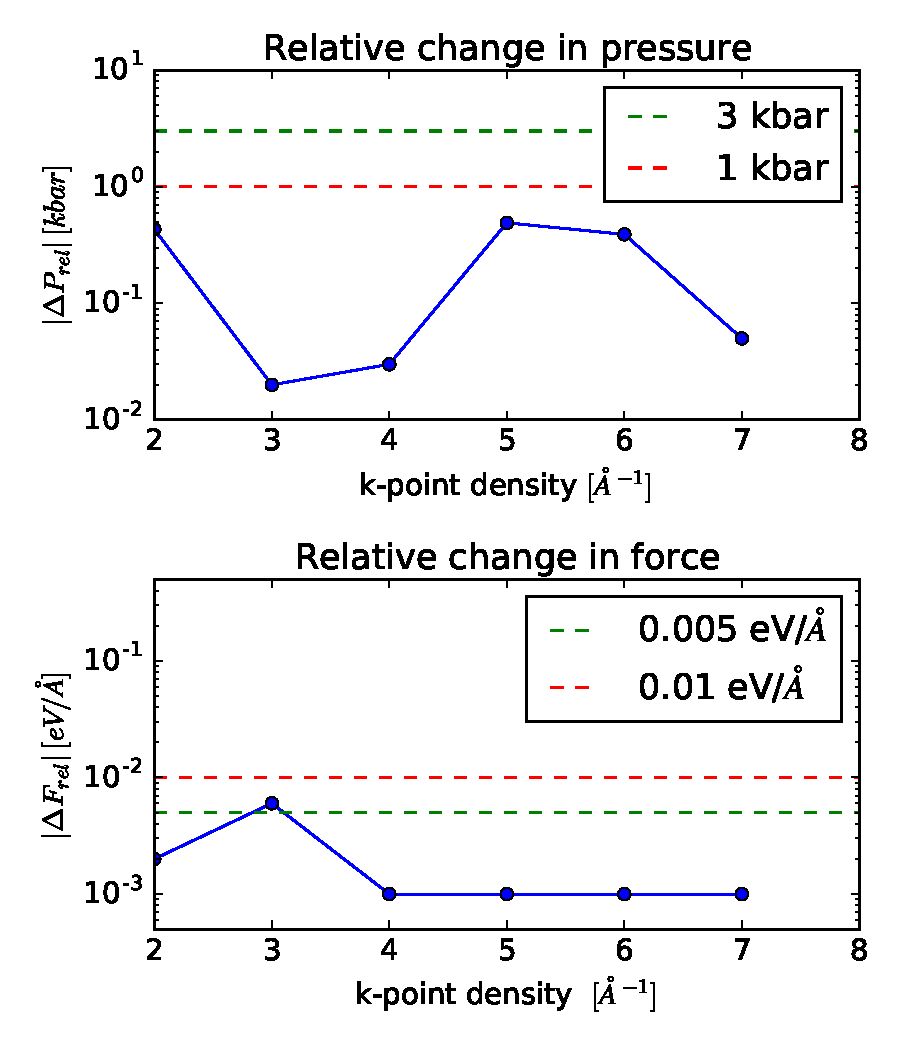
\includegraphics[width=\linewidth]{../fig/deltaforcepressrel_kpoints.pdf}\caption{This is a plot of the difference between change in both force and pressure for $\text{Ga}_2\text{O}_3$ with and without a oxygen vacancy. All the k-point densities gives good convergence.}\label{fig:forcepresskpoints}
\end{figure}

The k-point density was changed to 3 k-points per Å, when the cell size as increased to a super cell. 

\textit{Should I put this in another subsection with the super cell?}

\subsection{Primitive unit cell}

With the decided convergence criteria and the resulting energy cut-off and k-point density, we relaxed the primitive unit cell. Table \ref{tab:ionstep_primitive} shows both the maximum force and the pressure decreasing.

\begin{table}[H]\caption{This table lists the start and stop of the relaxation of the primitive unit cell. Both the maximum force, F$_{max}$, and the pressure, P, is decreasing in the relaxation.}\label{tab:ionstep_primitive}
\begin{tabular}{rllll}
F$_{max}$ &\#$_{atom}$&	P&	Drift&	E$_{tot}$\\ \hline
1.716&	9&	139.52&	0.000&	-119.461\\
$\vdots$&$\vdots$&$\vdots$&$\vdots$&$\vdots$\\
0.006&	9&	0.42&	0.000&	-120.224\\ \hline
CPU &time: & & & 685.881 s \\
\end{tabular}
\end{table}

The total energy per atom with a primitive unit cell was $\frac{E_{tot}}{\# \text{of atoms}} = \frac{•}{•}$ after the relaxation.

\subsubsection{Density of States}

To examine the different oxygen sites, the local density of state for the inequivalent sites were plotted in Figures \ref{fig:ldos_Ga_I} to \ref{fig:ldos_O_III} the total density of state of the primitive unit cell is plotted in Figure \ref{fig:total_dos_primitive}.

\begin{figure}[H]
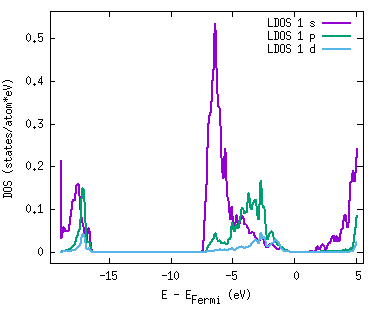
\includegraphics[width=\linewidth]{../fig/dosplot/ldos_Ga_I}\caption{This is a plot of local density of state at the Ga(I) site.}\label{fig:ldos_Ga_I}
\end{figure}

\begin{figure}[H]
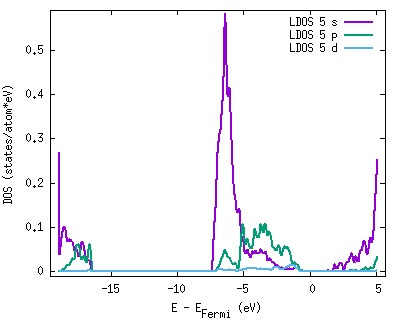
\includegraphics[width=\linewidth]{../fig/dosplot/ldos_Ga_II}\caption{This is a plot of local density of state at the Ga(II) site.}\label{fig:ldos_Ga_II}
\end{figure}

\begin{figure}[H]
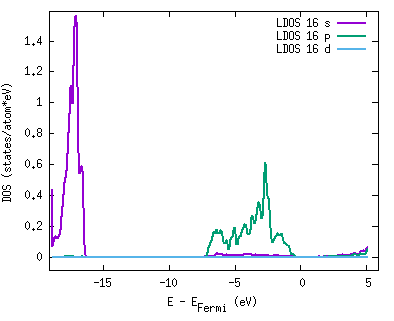
\includegraphics[width=\linewidth]{../fig/dosplot/ldos_O_I}\caption{This is a plot of local density of state at the O(I) site.}\label{fig:ldos_O_I}
\end{figure}

\begin{figure}[H]
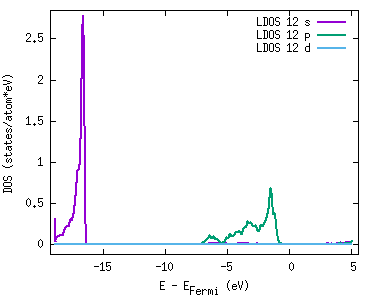
\includegraphics[width=\linewidth]{../fig/dosplot/ldos_O_II}\caption{This is a plot of local density of state at the O(II) site.}\label{fig:ldos_O_II}
\end{figure}

\begin{figure}[H]
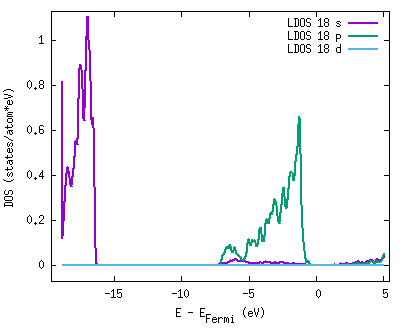
\includegraphics[width=\linewidth]{../fig/dosplot/ldos_O_III}\caption{This is a plot of local density of state at the O(III) site.}\label{fig:ldos_O_III}
\end{figure}

\begin{figure}[H]
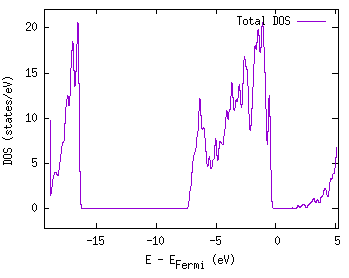
\includegraphics[width=\linewidth]{../fig/dosplot/total_dos_primitive_unitcell}\caption{This is a plot of density of state of the primitive unit cell.}\label{fig:total_dos_primitive}
\end{figure}

In the section about the structure we can see that all the oxygen sites are 'bonded' to both gallium sites, but the number of each bonds differ. We can see the p-orbitals with energy, $E-E_{Fermi}$, form -15 eV to 0 eV in all the local density plots indicating bonds between them all. There is also s-orbitals below -17 eV, but it is very small for the gallium atoms.


\subsubsection{Band structure}

Should do INCAR$_{dos}$ again with ISMEAR -5?

At last we plotted the band structure of $\beta$-Ga$_2$O$_3$ the band gap was found to be 1.8051 eV which is way to small, but a too small band gap is a common error with the simple functionals we are using in this project. Figure \ref{fig:bandstructure_primitive} shows the band structure we plotted after our calculations. Figure \ref{fig:bandstructure_fasit} shows the band structure from an article where they used hybrid functionals and other tricks to get the correct band gap \cite{dft_ga2o3}. 

The band structure in Figure \ref{fig:bandstructure_primitive} shows that the lowest point in the conduction band is at the $\Gamma$-point (G), and this corresponds with the result in Figure \ref{fig:bandstructure_fasit}. The highest point in the valence band on our band structure is difficult to set, but in the other it is either at the M-point or the $\Gamma$-point.

There seems to be something wrong at the M-point in our calculations because it looks very different form the other one. The band gap of $\beta$-Ga$_2$O$_3$ is indirect, but the difference in the valence band between the $\Gamma$-point and the M-point is so small, that it is practically direct.

\textit{Some more stuff in the discussion?}

\begin{figure}[H]\caption{This is a plot of the band structure of $\beta$-Ga$_2$O$_3$ form our density of states calculations.}\label{fig:bandstructure_primitive}
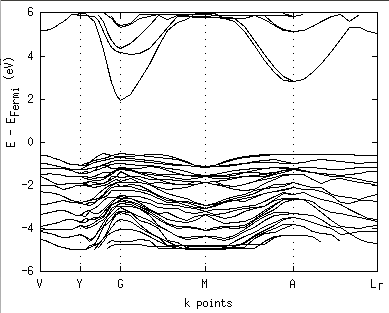
\includegraphics[width=\linewidth]{../fig/primitive/bandstructure}
\end{figure}


\begin{figure}[H]\caption{This is a plot of the band structure taken from an article that did DFT on $\beta$-Ga$_2$O$_3$ with hybrid density functionals \cite{dft_ga2o3}.}\label{fig:bandstructure_fasit}
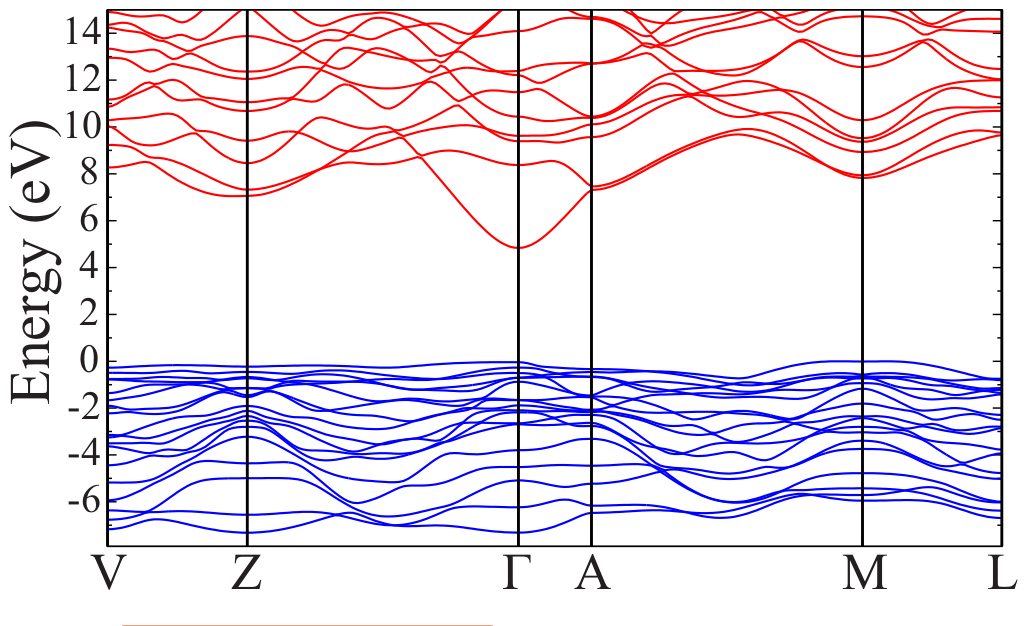
\includegraphics[width=\linewidth]{../fig/band_structure}
\end{figure}


\subsection{Supercell}

\subsubsection{Relaxation and energy}

Energy cut-off: 600 eV

K-mesh: 3x4x3

EDIFFG = -0.05

ISIF = 2

\begin{table}[H]\caption{The ionstep - relaxation of supercell with convergence result.}\label{tab:ionstep_convergence}
\begin{tabular}{rllll}
F$_{max}$ &\#$_{atom}$&	P&	Drift&	E$_{tot}$\\ \hline
0.443&	49&	134.07&	0.023&	-718.260\\
$\vdots$&$\vdots$&$\vdots$&$\vdots$&$\vdots$\\
0.009&	25&	109.22&	0.023&	-718.913\\ \hline
CPU &time: & 3546.421 s & & $\approx$ 59 min  \\
\end{tabular}
\end{table}

Energy calculation after:
\begin{table}[H]\caption{The energy output after relaxation of supercell.}\label{tab:energy_supercell_after_relax}
\begin{tabular}{llll}
F$_{max}$ & P&	Drift&	E$_{tot}$\\ \hline
0.045&	0.023&	2.63	& \ref. \\
\end{tabular}
\end{table}

\subsubsection{Changed convergence criteria}

To have less CPU time with super cell I lowered the criteria to:

Energy cut-off: 500 eV

K-mesh: 2x3x2 (density 3)

EDIFFG = -0.01

ISIF = 3

\begin{table}[H]\caption{The ionstep - relaxation of supercell with convergence result.}\label{tab:ionstep_convergence}
\begin{tabular}{rllll}
F$_{max}$ &\#$_{atom}$&	P&	Drift&	E$_{tot}$\\ \hline
0.427&	49&	136.09&	0.023&	-717.821\\
$\vdots$&$\vdots$&$\vdots$&$\vdots$&$\vdots$\\
0.006&	49&	0.03&	0.024&	-720.914\\ \hline
CPU &time: &  1763.585 s & & $\approx$ 29 min  \\
\end{tabular}
\end{table}

Energy calculation after:
\begin{table}[H]\caption{The energy output after relaxation of supercell.}\label{tab:energy_supercell_after_relax}
\begin{tabular}{llll}
F$_{max}$ & P&	Drift&	E$_{tot}$\\ \hline
0.045&	0.023&	2.63	&-721.081\\
\end{tabular}
\end{table}


\subsection{O$_2$ in vacuum}

Describe the INCAR file - what is different in this then the other ones? In theory?

\begin{table}[H]\caption{The energy output of oxygen in vacuum.}\label{tab:oxygen_vacuum}
\begin{tabular}{llll}
F$_{max}$ &	P&	Drift&	E$_{tot}$ \\ \hline
0.088&	0.000&	-0.22&	-9.883\\
\end{tabular}
\end{table}

\subsubsection{Chemical potential}

%$$ \mu_{O_2} = E^{tot}_{O_2} + \tilde{\mu}_{O_2}(T,p^0) + kT \ln (p/p^0)$$

$$ \mu_O = \frac{1}{2}\mu_{O_2} = \frac{1}{2}\cdot(-9.883) = -4.942 $$

\subsection{Different oxygen vacancies}

\subsubsection{O(I) vacancy}


\begin{table}[H]\caption{The ionstep - relaxation of super cell with O(I) vacancy.}\label{tab:ionstep_O_I}
\begin{tabular}{rllll}
F$_{max}$ &\#$_{atom}$&	P&	Drift&	E$_{tot}$\\ \hline
2.666&	19&	133.08&	0.142&	-708.492\\
$\vdots$&$\vdots$&$\vdots$&$\vdots$&$\vdots$\\
0.032&	63&	-0.03&	0.465&	-712.142\\ \hline
CPU &time: & & & 5127.663 s \\
& & & &$\approx$ 1 t 25 min\\
\end{tabular}
\end{table}

\subsubsection{O(II) vacancy}

\begin{table}[H]\caption{The ionstep - relaxation of super cell with O(II) vacancy.}\label{tab:ionstep_O_II}
\begin{tabular}{rllll}
F$_{max}$ &\#$_{atom}$&	P&	Drift&	E$_{tot}$\\ \hline
2.391&	20&	135.21&	0.010&	-708.256	\\
$\vdots$&$\vdots$&$\vdots$&$\vdots$&$\vdots$\\
0.013&	60&	-0.01&	0.143&	-711.709\\ \hline
CPU &time: & & &  5061.359 s \\
\end{tabular}
\end{table}


\subsubsection{O(III) vacancy}

\begin{table}[H]\caption{The ionstep - relaxation of super cell with O(III) vacancy.}\label{tab:ionstep_O_III}
\begin{tabular}{rllll}
F$_{max}$ &\#$_{atom}$&	P&	Drift&	E$_{tot}$\\ \hline
1.873&	1&	135.42&	0.141&	-707.966	\\
$\vdots$&$\vdots$&$\vdots$&$\vdots$&$\vdots$\\
0.017&	73&	-0.00&	0.145&	-711.463	\\ \hline
CPU &time: & & & 5115.230 s \\
\end{tabular}
\end{table}

\subsubsection{Total Energy}

\begin{table}[H]\caption{The energy output after relaxation of supercell with oxygen vacancies.}\label{tab:energy_supercell_vacancies}
\begin{tabular}{lllll}
Vacancy& F$_{max}$ &	P&	Drift&	E$_{tot}$ \\ \hline
O(I)&    0.107&	    0.146&	2.29	&    -712.283\\
O(II)&    0.067&	    0.198&	2.39	&    -711.860\\
O(III)&    0.087&    0.221&	2.13	&    -711.603\\
\end{tabular}
\end{table}


\subsubsection{Formation Energy}

$$E^f = E_d - E_h - \sum_i \Delta n \mu_i = E_d - E_h - \mu_O$$

\begin{table}[H]\caption{This is the calculated formation energies for the diffrent oxygen vacancies at oxygen rich conditions.}\label{tab:energy_formation}
\begin{tabular}{cc}
Vacancy& E$_b$ - (E$_{vac}$ + $\mu_O$) = E$_f$ \\ \hline
O(I)&  -721.081 - (-712.282 -4.942) = -3.857\\
O(II)&  -721.081 - (-711.860 -4.942) = -4.279\\
O(III)&  -721.081 - (-711.603 -4.942) = -4.536\\
\end{tabular}
\end{table}

\subsection{Why the O(I) vacancy?}

\newpage

\subsubsection{Total density of states}

Notice the new level in the band gap - defect level - filled.

\begin{figure}[H]
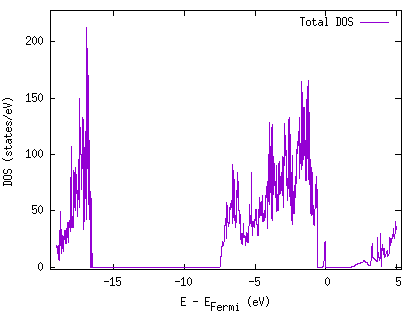
\includegraphics[width=\linewidth]{../fig/dosplot/total_dos_O_I_vacancy}\caption{This is a plot of the density of state of the super cell with a O(I) vacancy.}\label{fig:total_dos_vac}
\end{figure}

\begin{figure}[H]
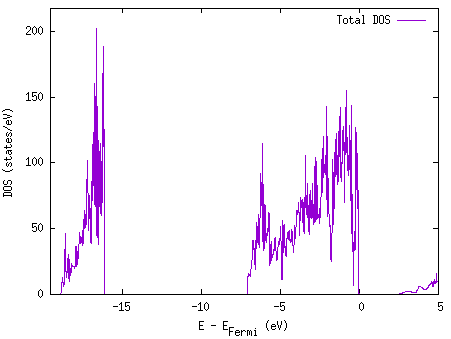
\includegraphics[width=\linewidth]{../fig/dosplot/total_dos_supercell}\caption{This is a plot of density of state of the general supercell.}\label{fig:total_dos_supercell}
\end{figure}

\subsubsection{Isosurfaces}

\paragraph*{O(I)}

\begin{figure}[H]
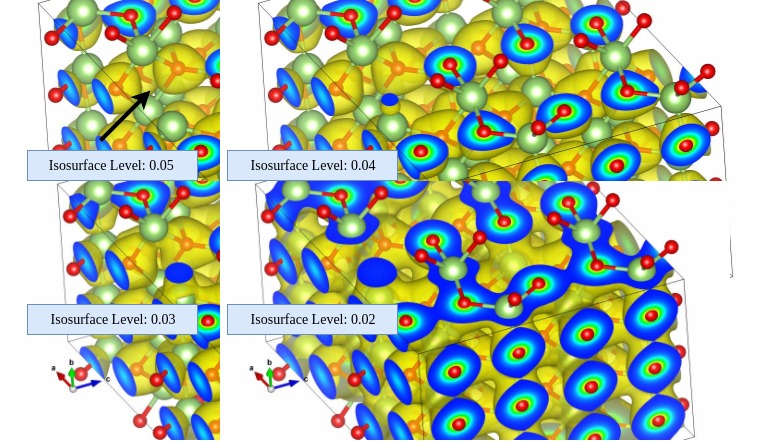
\includegraphics[width=\linewidth]{../fig/isosurfaces/O_I/isosurface}\caption{This figure shows the oxygen vacancy with different isosurfaces.}\label{fig:isosurface_O_I}
\end{figure}


\paragraph*{O(I)}


\paragraph*{O(II)}

\subsubsection{Local DOS Ga(II)}

\begin{figure}[H]
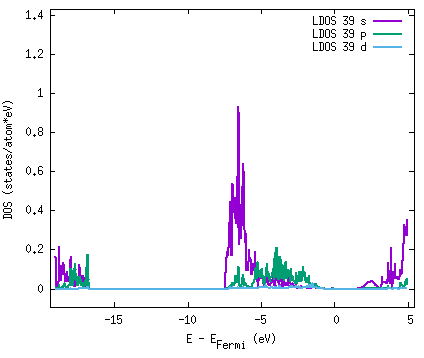
\includegraphics[width=\linewidth]{../fig/dosplot/ldos_Ga_II_OI_vac_nabo}\caption{This is a plot of local density of state at the Ga(II) site next to the O(I) vacancy in the super cell.}\label{fig:ldos_Ga_II_nabo}
\end{figure}

\begin{figure}[H]
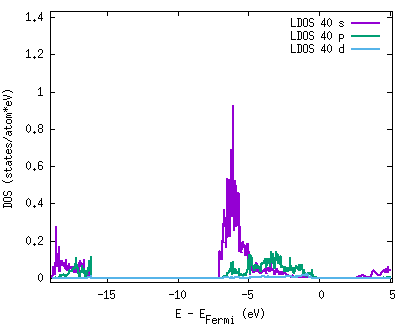
\includegraphics[width=\linewidth]{../fig/dosplot/ldos_Ga_II_supercell}\caption{This is a plot of local density of state at the Ga(II) site in the general supercell.}\label{fig:ldos_Ga_II_supercell}
\end{figure}

\subsubsection{Local DOS Ga(I)$_1$}

\begin{figure}[H]
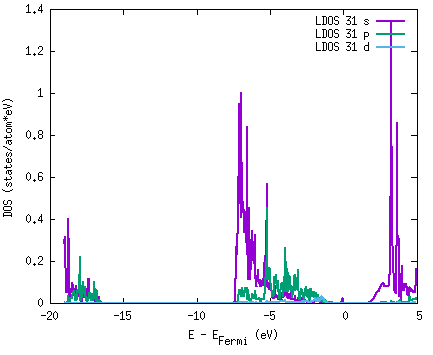
\includegraphics[width=\linewidth]{../fig/dosplot/ldos_Ga_I_OI_vac_nabo}\caption{This is a plot of local density of state at the Ga(I) site next to the O(I) vacancy in the super cell.}\label{fig:ldos_Ga_I_nabo}
\end{figure}

\begin{figure}[H]
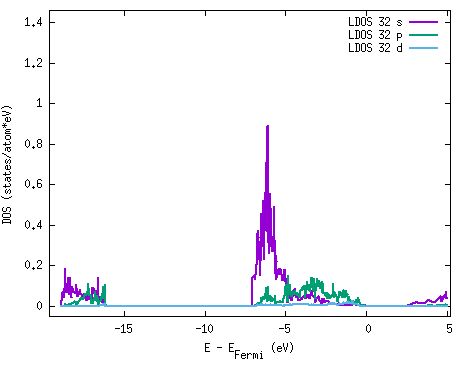
\includegraphics[width=\linewidth]{../fig/dosplot/ldos_Ga_I_supercell}\caption{This is a plot of local density of state at the Ga(I) site in the general supercell.}\label{fig:ldos_Ga_I_supercell}
\end{figure}

\subsubsection{Bond between Ga(I)$_1$ and Ga(I)$_2$?}

\begin{figure}[H]
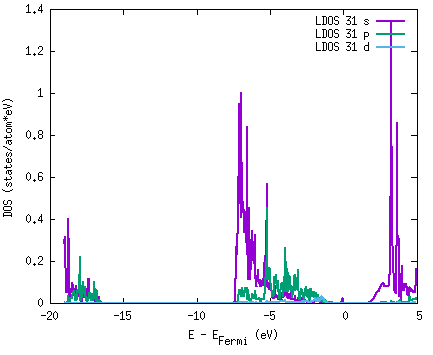
\includegraphics[width=\linewidth]{../fig/dosplot/ldos_Ga_I_OI_vac_nabo}\caption{This is a plot of local density of state at the Ga(I) site next to the O(I) vacancy in the super cell.}\label{fig:ldos_Ga_I_nabo}
\end{figure}

\begin{figure}[H]
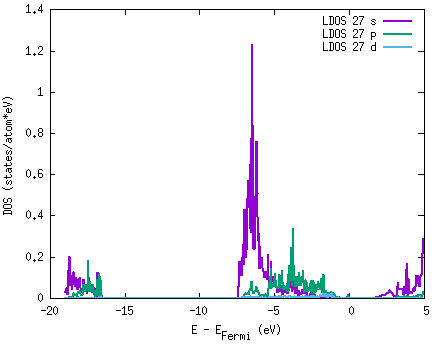
\includegraphics[width=\linewidth]{../fig/dosplot/ldos_Ga_I_OI_vac_nabo2}\caption{This is a plot of local density of state at the other Ga(I) site next to the O(I) vacancy in the super cell.}\label{fig:ldos_Ga_I_nabo}
\end{figure}

